\documentclass[a4paper, 12pt]{article}
\usepackage[top=2cm, bottom=2cm, left=2.5cm, right=2.5cm]{geometry}
\usepackage[utf8]{inputenc}
\usepackage[brazilian]{babel}
\usepackage{indentfirst}
\usepackage{graphicx}
\usepackage{wrapfig}
\usepackage[pdftex]{hyperref}
\usepackage{amsmath}

\begin{document}
	\begin{center} %centralizar o texto abaixo
		{\Large Reposta de um sistema de segunda ordem ao degrau}\\[0.4cm]
		{\large Erik Yuji Goto}\\[0.2cm]
		{\normalsize RA: 234009}
	\end{center} %término do comando centralizar

\section{Modelagem no Simulink}
\subsection{Diagrama de Blocos no Simulink}
Para iniciar nossa resolução vamos reorganizar a equação diferencial($m\ddot{x} + c\dot{x} + kx = f(t)$) e substituir com os valores do enunciado:
\begin{figure}[h]
		\center
		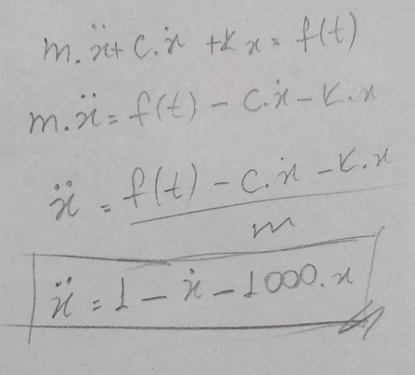
\includegraphics[scale=0.6]{Imagens/aa.png}
		\caption{Equação Diferencial}
	\end{figure}
	\\
Portanto,
\begin{figure}[h]
		\center
		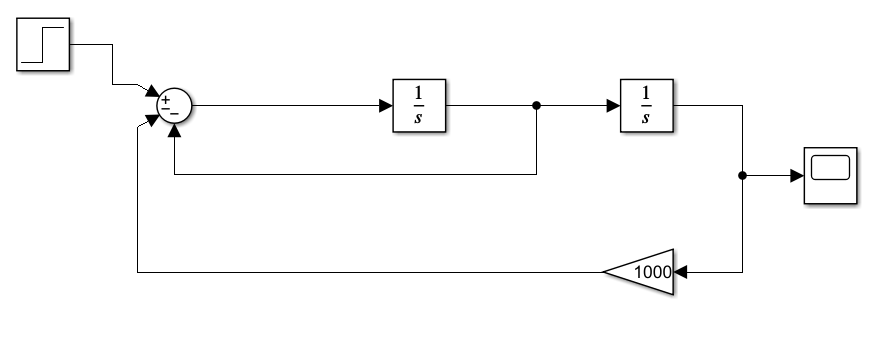
\includegraphics[scale=0.6]{Imagens/aaa.png}
		\caption{Diagrama de Blocos}
	\end{figure}
\begin{equation}
	\ddot{x} = 1 - \dot{x} - 1000 x
\end{equation}
Com a função \textit{Scope} conseguimos visualizar a solução:
\begin{figure}[h]
		\center
		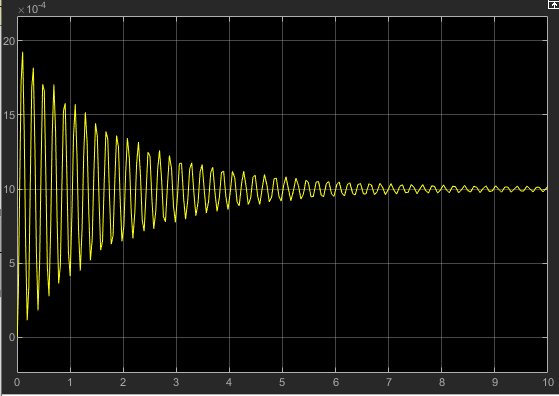
\includegraphics[scale=0.6]{Imagens/scope.png}
		\caption{Scope - diagrama de blocos}
	\end{figure}

\newpage
\subsection{Função Transferência}
	Outra forma de resolver a equação no Matlab é pela função transferência. Para começar vamos calcular a função de transferência:
	\begin{figure}[h]
		\center
		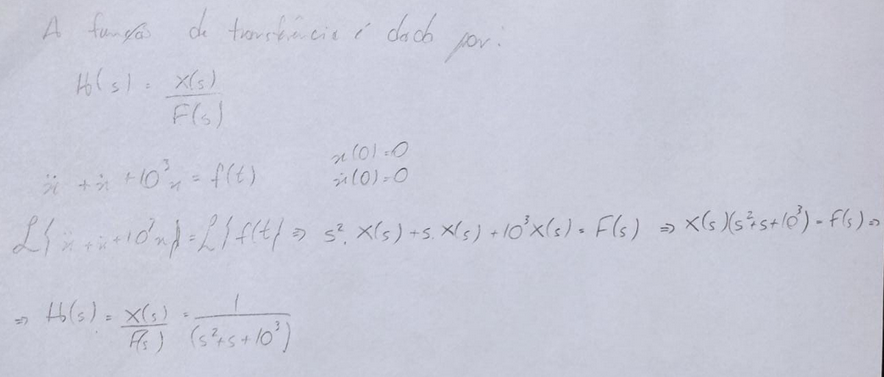
\includegraphics[scale=0.6]{Imagens/ft.png}
		\caption{Cálculo da Função Transferência}
	\end{figure}
	\\
	Ou seja,
	\begin{equation}
		H(s) = \frac{1}{s^2 + s + 10^3}
	\end{equation}
	
	Para usar a função transferência no simulink usamos o bloco \textit{Transfer Fcn}
	\begin{figure}[h]
		\center
		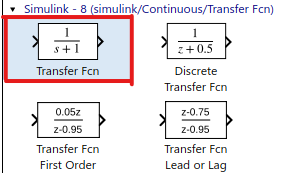
\includegraphics[scale=0.7]{Imagens/ft_s.png}
		\caption{Funcção Transferencia no Simulink}
	\end{figure}\\
	E a simulação completa fica da seguinte forma:
	\begin{figure}[h]
		\center
		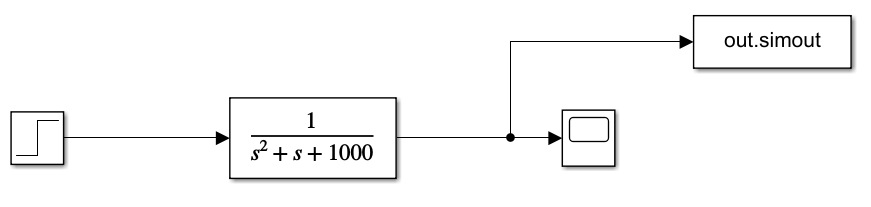
\includegraphics[scale=0.5]{Imagens/sim.png}
		\caption{Simulação no Simulink}
	\end{figure}
	\begin{figure}[h]
		\center
		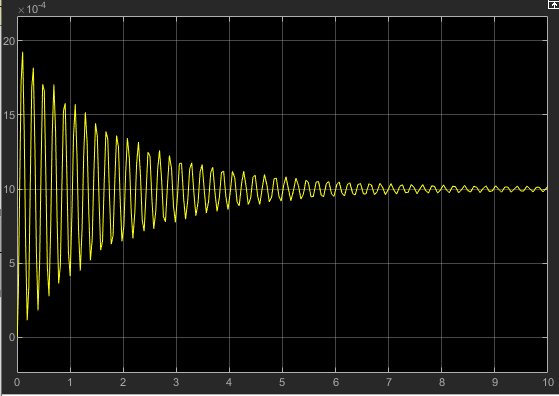
\includegraphics[scale=0.5]{Imagens/scope.png}
		\caption{Scope - função transferência}
	\end{figure}\\
Note que, a saída do scope retornou exatamente o mesmo gráfico ao usar o diagram de blocos e o bloco transferência.
\newpage
\section{Solução Analítica - Transformada de Laplace}
	Outra maneira de resolver a equação diferencial é por meio da \textit{Transformada de Laplace}:
	\begin{figure}[h]
		\center
		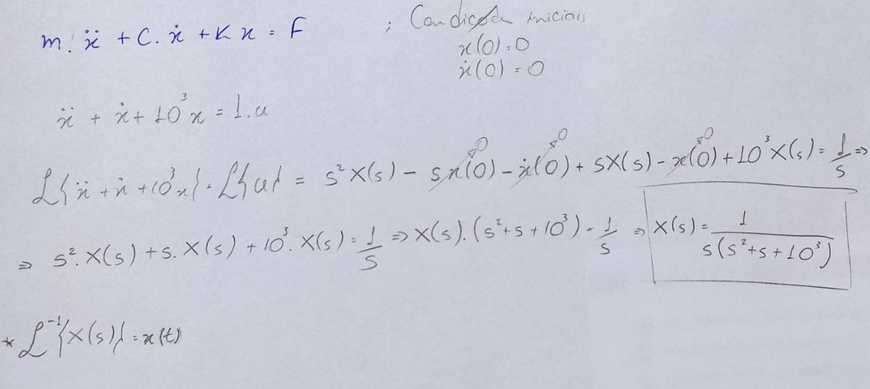
\includegraphics[scale=0.55]{Imagens/la.png}
		\caption{Solução por Laplace}
	\end{figure}\\
	Onde chegamos a:
	\begin{equation}
		X(s) = \frac{1}{s(s^2 + s + 10^3)}
	\end{equation}
	Calculamos a anti-transformada (2) com o auxílio do \textit{MatLab}:
	\begin{figure}[h]
		\center
		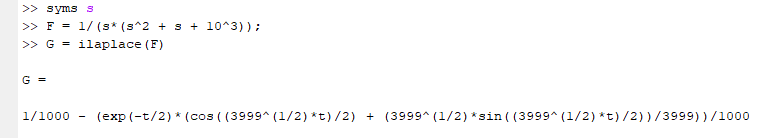
\includegraphics[scale=0.7]{Imagens/ma.png}
		\caption{Anti-transformada}
	\end{figure}
	\newpage
	Portanto,\\
	\begin{equation}
		G = x(t) = \frac{1}{1000} - (e^{-t/2}(cos(\frac{(3999^{1/2}t)}{2}) + 3999^{1/2}\frac{sen(\frac{3999^{1/2}t}{2})}{3999}))/1000
	\end{equation}
	Agora que temos $x(t)$ conseguimos plotar o gráfico da solução analítica:
	\begin{figure}[h]
		\center
		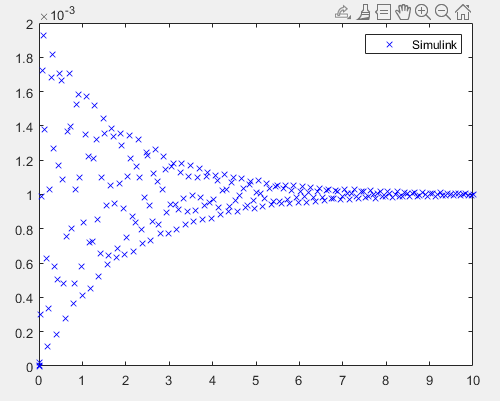
\includegraphics[scale=0.8]{Imagens/a.png}
		\caption{Gráfico da solução analítica}
	\end{figure}	 
	
	\newpage
\section{Análise dos Resultados}
	Para comparar as duas soluções vamos plotar em um único gráfico:
	\begin{figure}[h]
		\center
		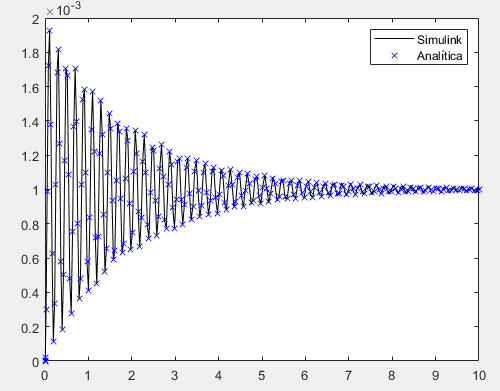
\includegraphics[scale=0.6]{Imagens/comp.png}
		\caption{Comparação entre as duas soluções}
	\end{figure}
	\begin{figure}[h]
		\center
		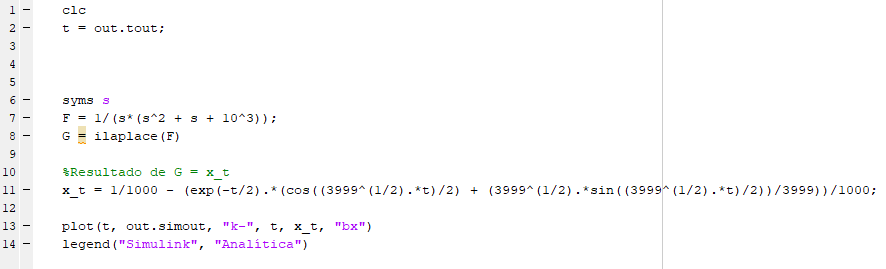
\includegraphics[scale=0.6]{Imagens/matt.png}
		\caption{Código no Matlab}
	\end{figure}
	
	
	
	
	
	
	
	
	
\end{document}